\chapter{Planning of the Bachelor Thesis}
\label{chap:planning}
\setstretch{1.25}

To have small and achievable goals to work on during the Bachelor Thesis, the project is divided in several milestones. In this chapter these milestones are listed and explained in detail on what is the goal, what are the methods used to achieve it, how is it tested and how to proof that they worked. The milestones will start from a few that are necessary to have the bare minimum done and will go up until the optimal solution. After the milestones were described, predictions are made on how far the project will be solved under different circumstances (e.g. worst-case scenario, no problems etc.).

\section{Milestone 1: Running programming environment}
\label{chap:mile1}
\subsubsection{Description}
Until this point of time, the work for this project was completely done on private systems of the student. As mentioned in chapter 4 a laptop was provided by the AHB. Since it is a school laptop, a Windows system is installed. In order to not uninstall the Windows off the Laptop, an external SSD was provided which should be configured to act as a bootable Ubuntu 18.04 Bionic Beaver System. Therefore, the system will start again from a clean installation and all needed libraries will be installed on to this system.
\subsubsection{Goal}
The Goal is straightforward to have a running programming environment which has all needed libraries and programs installed.
\subsubsection{Methods used to achieve the goal}
Following installation instructions of different libraries which are offered by the providers of the needed libraries.
\subsubsection{Testing}
Ubuntu is bootable from multiple Devices.
The boot will be tested on at least two different devices. 
\subsubsection{Validation and proof}
The device allows a flawless boot of the Ubuntu into the desired home screen without changing the predefined setups.
Proof is a written statement of the user / author.

\section{Milestone 2: Robot communication}
\label{chap:mile2}
\subsubsection{Description}
Without the communication with the robot, the task of the project can't be achieved. Therefore it is very important to set up a stable connection and communication from the system to the robot in order to provide each side of the system with the necessary data.
\subsubsection{Goal}
Flawless communication between collision avoidance system and robot.
\subsubsection{Methods used to achieve the goal}
Review the example provided over git and the socket messaging method already in use at AHB. Work with the Fanuc manual in order to set up the communication.
\subsubsection{Testing}
In order to test the communication, a simple C++ program should be able to feed the robot Cartesian or joint coordinates to move to. The robot shall move accordingly.
\subsubsection{Validation and proof}
The C++ as well as the Karel code shall be pushed to git in a separate folder, to provide a simple example for future communication tasks.
A video shall be provided as proof for the functioning communication. The video shall show the execution of the C++ code and the robot's movements. The video and the source code will be committed in a single commit in order to have a  clear identification.

\section{Milestone 3: Scanning of the workspace}
\label{chap:mile3}
\subsubsection{Description}
The cameras shall be implemented into the system and a point cloud of the Workspace shall be created. The data shall be processed into a two-dimensional occupancy grid for a first simple motion planner.
\subsubsection{Goal}
Visualizing the workspace in form of a point cloud and an occupancy grid.
\subsubsection{Methods used to achieve the goal}
Using the Point Cloud Library, the cameras shall be implemented. Since the PCL supports either Microsoft Kinect or Asus Xtion Pro, both cameras may be used, the one with the better resulsts shall be used for the rest of the project.
\subsubsection{Testing}
In order to test the task, the workspace shall be changed by placing different objects on various points inside the workspace.
Point clouds and occupancy grids will be reviewed manually and checked for their accuracy.
\subsubsection{Validation and proof}
The successful test will be proceeded and documented with both kinds of cameras.
The resulting grids are analyzed manually and a ranking for completeness and accuracy will be done.
Proof shall be provided over screenshots and written comments of the observation and usability of the author.

\section{Milestone 4: Simple 2D Motion Planning, End-Effector only}
\label{chap:mile4}
\subsubsection{Description}
In a first collision avoidance step, the robot shall move around objects in a static two dimensional environment. This means during robot movements the workspace shall not change. A simple algorithm for path planning is the PRM algorithm, which should be available over the Open Motion Planning Library. PRM is already known since it was used during the robotics 2 course. In this course an implementation was realized over Matlab.
\subsubsection{Goal}
Move from start position to given goal position without any collision.
\subsubsection{Methods used to achieve the goal}
The point clouds gathered from the cameras using PCL, shall be processed into an 2D occupancy grid using OctoMap. The probabilistic road map planner (PRM) uses occupancy grids and places nodes inside the map on randomly chosen free cells. The nearest nodes to the starting and goal location are searched. Then a path along the nodes is calculated and thus provides a path from start to goal position. The PRM planner can be used from the OMPL library.
This step plans the motions only for the end-effector, which means the robot arm needs to remain elevated over the obstacles in order to remain collision free. Therefor movements can only be made in the XY-plane in Cartesian space.
\subsubsection{Testing}
By changing the workspace with different objects on various places, the map generation and the path planning shall be tested. The starting position shall be read from the Karel code as the current robot position, the goal position shall be provided over the C++ Code as an user input.
\subsubsection{Validation and proof}
Three successful test runs with different objects in different positions and variable start and end points shall be proceeded.
A video of the robot's movement around the object shall be made for every run to proof that the path planning works in different test set-ups.

\section{Milestone 5: Simple 3D Motion Planning, End-Effector only}
\label{chap:mile5}
\subsubsection{Description}
As a second collision avoidance step, the robot shall move around in a static three dimensional environment. The objects inside the workspace shall remain static during robot movements. For the motion planning, again the PRM algorithm shall be used, but this time in a 3D space.
\subsubsection{Goal}
Move from start position to given goal position without any collision in the three dimensional space.
\subsubsection{Methods used to achieve the goal}
The point clouds gathered from the cameras using PCL, shall be processed into an 3D occupancy grid using OctoMap. Using the PRM planner from OMPL a path from start to goal shall be calculated and afterwards moved along with the robot.
This step plans the motions only for the end-effector, which means the robot arm needs to remain elevated over the obstacles in order to remain collision free. Therefor movements can only be made in the Cartesian space.
\subsubsection{Testing}
By changing the workspace with different objects on various places, the map generation and the path planning shall be tested. The starting position shall be read from the Karel code as the current robot position, the goal position shall be provided over the C++ Code as an user input.
\subsubsection{Validation and proof}
Three successful test runs with different objects in different positions and variable start and end points shall be proceeded.
A video of the robot's movement around the object shall be made for every run to proof that the path planning works in different test set-ups.

\section{Milestone 6: Collision detection for whole robot model}
\label{chap:mile6}
\subsubsection{Description}
The next step to improve the collision avoidance system shall provide a collision detection not only for the end-effector but for the whole robot model. This shall be achieved by creating a occupancy grid for the robot model and its trajectories. By comparing the two different grids (workspace and robot) collisions shall be predicted and avoided.
\subsubsection{Goal}
Find or create a motion planner who is able to calculate a path based on swept volumes. 
Move from start position to given goal position without any collision, movements can be done in joint space or Cartesian space.
\subsubsection{Methods used to achieve the goal}
A 3D model of the robot provides the base for the robot occupancy grid. Using the joint speeds, a prediction of the joint positions can be calculated and swept volumes can be created inside the occupancy grid. Both occupancy grids shall be compared by simply checking if a cell is occupied in both grids. The cells which are occupied in both grids show a collision that needs to be avoided.
To have a proper motion planning algorithm based on these data, further literature review is necessary.

\subsubsection{Testing}
The workspace shall be changed for different motions by placing various objects in different positions. In order to test the collision detection for the robot arm, objects shall be placed in front of the arm to force a movement to avoid the collision not only of the end-effector.

\subsubsection{Validation and proof}
Three successful test runs with different objects in different positions and variable start and end points shall be proceeded.
A video of the robot's movement around the object shall be made for every run to proof that the path planning works in different test set-ups.

\section{Milestone 7: Collision detection in a dynamic workspace}
\label{chap:mile7}
\subsubsection{Description}
The previously used motion planner shall be adapted to work in a dynamic workspace (e.g. moving objects, humans). The movements of the robot shall be adapted in real time to avoid collisions. The results of the collision avoidance system shall be visualized in a GUI. 


\subsubsection{Goal}
Robot moves from start to goal location in a dynamic workspace, without any collisions.
Implement a GUI to show the results of the collision avoidance system.

\subsubsection{Methods used to achieve the goal}
The workspace shall be monitored in real-time, updating occupancy grids on the fly. The motion planner should work with the permanently updating occupancy grids in order to react to dynamic obstacles.
Further literature review is necessary to achieve this goal.

\subsubsection{Testing}
In a first phase, object shall be moved inside the workspace, using objects which can be moved from outside of the workspace to reduce risks for humans.
In a second phase, when the system has a high level of success an values can be considered as trustworthy, humans shall enter and leave the workspace in order to simulate a walk by.

\subsubsection{Validation and proof}
Six successful test runs with different objects in various positions and variable start and end points shall be proceeded by using objects which are moved from outside of the workspace.
A video of the robot's movement around the object shall be made for every run to proof that the path planning works in different test set-ups. 
After the successful first testing phase another three test runs with humans shall be proceeded and recorded on video. 

\section{Prediction}

Milestones one to four are defined as bare minimum, as these are the necessary milestones to have a first path planning based on the sensor data, which implements a first step of the collision avoidance system. Based on the actual knowledge it should be possible to reach Milestone six within the given eight weeks of the Bachelor Thesis. If progress during the work is exceptionally good, even milestone seven can be reached.

To prevent the lost of track, an escalation to the experts is needed, whenever the forseen timeline of the worst case is not fulfilled. This would mean, that the minimal goal is threatened and a solution to this upcoming problem need to be found. In addition it helps the author to prevent losing focus as it happened in the preliminary study.

\begin{figure}[h]
	\begin{center}
		\centering
		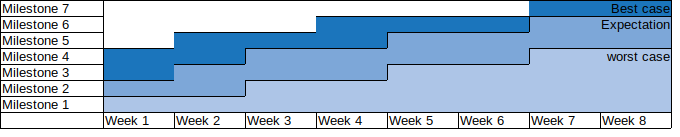
\includegraphics[width=1.0\linewidth]{images/Milestones.png}
		\caption{Milestones in Timeline}
		\label{fig:milestones}
	\end{center}
\end{figure}